\documentclass[11pt,a4paper]{article}
\usepackage[utf8]{inputenc}
\usepackage[spanish]{babel}
\usepackage{amsmath}
\usepackage{amsfonts}
\usepackage{amssymb}
\usepackage{makeidx}
\usepackage{graphicx}
\usepackage{lmodern}
\usepackage{kpfonts}
\usepackage[left=2cm,right=2cm,top=2cm,bottom=2cm]{geometry}
\author{Miguel Angel Xamie Diaz Fuentes}

\begin{document}
\begin{center}
\begin{LARGE}
\textbf{INGENIERÍA MECATRÓNICA}\\
\end{LARGE}
{\large Sistemas Eletrónicos De Interfaz}\\
\begin{figure}[hbtp]
\centering

\includegraphics[scale=0.80]{UPZMG_Mecatr_nica.png}
\end{figure} 
\begin{center}
\begin{LARGE}
EV-2-2-EXPLICAR LOS ARREGLOS Y PARAMETROS DE LOS AMPLIFICADORES CLASE A
\end{LARGE}
\end{center}

\begin{Large}
\textbf{Alumno}
\\\textit{Miguel Angel Xamie Diaz Fuentes}
\textbf{\\Maestro}
\\\textit{Morán Garabito Carlos Enriquez}
\textbf{\\Fecha de Entrega}
\\\textit{01/10/2019}
\textbf{\\Grupo}
\\\textit{4-B}
\end{Large}

\end{center}

\footnote{Universidad Politécnica De La Zona Metropolitana De Guadalajara} 

\newpage

\section{Desarrollo}

\begin{flushleft}
\textbf{Etapa de potencia, amplificador de potencia o etapa de ganancia} son los nombres que se usan para denominar a un amplificador de audio. La funcion del amplificador es aumentar el nivel de señal, incrementando para ella la amplitud de la señal de entrada mediante corrientes de polarización (voltaje negativo, voltaje positivo) en el transistor de salida.\\

EL amplificador trabaja, internamente, con corriente continua; en caso de ser alimentado con la tensión entregada por la red domiciliaria se necesita un transformador y rectificador para adaptar el nivel de voltaje y tipo de corriente a los valores necesarios para el buen funcionamiento del equipo.\\
\end{flushleft}

\textbf{Características Técnicas}\\

Las características técnicas de cada modelo determinarán la calidad del amplificador:\\

\begin{itemize}

\item Impedancia.\\
\item Factor de amortiguamiento.\\
\item Potencia de salida.\\
\item Relación señal ruido.\\
\item Acomplamiento.\\
\item Respuesta en frecuencia.\\
\item Respuesta de fase.\\
\item Ganancia.\\
\item Sensibilidad.\\
\item Distorsión.\\
\item Diafonía.\\

\subsection{Amplificador de Clase A}

La corriente de salida circula durante todo el cliclo de la señal de entrada, en un solo transistor. La corriente de polarización del transistor de salida es alta y constante durante todo el proceso, independiente de si hay o no hay salida de audio. La distorsión introducida es baja a niveles muy bajos de señales (para niveles altos las distorsiones de segundo orden son importantes), el rendimiento también será bajo, estando siempre por debajo del 50 por ciento, lo que significa que la otra mitad de la corriente amplificada será disipada por el transistor en forma de calor. 

\footnote{Universidad Politécnica De La Zona Metropolitana De Guadalajara} 

\newpage

Los amplificadores de clase A se utilizan solo en etapas preamplificadoras, su bajo rendimiento y su elevado nivel de distorsión armónica no lo hacen aptos para etapas de potencia. La curva de transferencia de un aumentando asi la capacidad lineal de transferencia (menor distorsiones, distorsiones de segundo orden casi nulas) y mayor eficiencia.

\begin{figure}[hbtp]
\centering
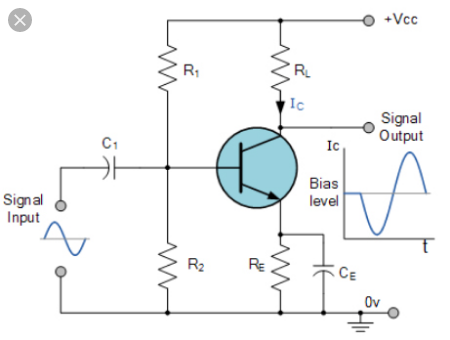
\includegraphics[scale=0.80]{ejemplo.png} 
\end{figure} 

Esta amplificación presenta el inconveniente de generar una fuerte y constante emisión de calor. No obstante, los transistores de salida están siempre a una temperatura fija y sin alteraciones.\\

En general, se afirma que esta clase de amplificación es frecuente en circuitos de audio y en los equipos domésticos de gama alta, ya que proporcionan una calidad de sonido potente y de muy buena calidad.\\

Los amplificador de clase A a menudo consisten en un transistor de salida conectado al positivo de la fuente de alimentación y un transistor de corriente constante conectado de la salida al negativo de la fuente de alimentación.\\

La señal del transistor de salida modula tanto el voltaje como la corriente de salida. Cuando no hay señal de entrada, la corriente de polarización constante fluye directamente del positivo de la fuente de alimentación al negativo, resultando que no hay corriente de salida, se gasta mucha corriente. Algunos amplificador de clase A más sofisticados tienen dos transistores de salida en configuración push-pull.\\

\footnote{Universidad Politécnica De La Zona Metropolitana De Guadalajara} 

\newpage

\textbf{VENTAJA}\\

La clase A se refiere a una etapa de salida con una corriente de polarización mayor que la máxima corriente de salida que dan, de tal forma que los transistores de salida siempre están consumiendo corriente. La gran ventaja de la clase A es que es casi lineal, y en consecuencia la distorsión es menor.\\

\textbf{DESVENTAJA}\\

La gran desventaja de la clase A es que es poco eficiente, se requiere un amplificador de clase A muy grande para dar 50 W, y ese amplificador usa mucha corriente y se pone a muy alta temperatura.\\

En los amplificadores de clase A no hay nunca corriente de reja (base) por lo que es indiferente decir que el amplificador es de clase A1 o de clase A. Lo contrario ocurre en los amplificadores de clase C donde siempre va a existir corriente de reja (base), en este caso es indiferente decir que el amplificador es de clase C2 o de clase C (a secas).


\end{itemize} 

\newpage


\bibliography{Referencia}
\begin{thebibliography}{X}
\bibitem{Baz} \textsc{RUMSEY, FRANCIS Y MCCORMICK, TIM.} \textit{Sonido y grabación. Introducción las técnicas sonoras.} IORTV, Segunda edición, 2004.

\bibitem{Baz} \textsc{MARKUS, JOHN.} \textit{Manual de Circuitos Electrónicos.} 
Alfaomega, Marcombo.


\bibitem{Baz} \textsc{LUIS GONZALES.} \textit{Amplificadores de potencia: Clasificación, tipos.} 
Electrónica Unicrom, 2006.
\end{thebibliography}

\bibliographystyle{plain}





\end{document}